\documentclass[12pt]{article}
\usepackage{subfiles}
\usepackage{graphicx}
\usepackage[
        pdfencoding=auto,%
        pdfauthor={Scott Pratt},%
        pdfstartview=FitV,%
        colorlinks=true,%
        linkcolor=blue,%
        citecolor=blue, %
        urlcolor=blue,
        breaklinks=true]{hyperref}
%\usepackage[anythingbreaks,hyphenbreaks]{breakurl}
\usepackage[anythingbreaks,hyphenbreaks]{xurl}
%\usepackage{pdfsync}
\usepackage{amssymb}
\usepackage{amsmath}
\usepackage{bm}
\numberwithin{equation}{section} 
\numberwithin{figure}{section} 
\usepackage[small,bf]{caption}
%\usepackage{fontspec}
%\usepackage{textcomp}
%\usepackage{color}
\usepackage{fancyhdr}
\setlength{\headheight}{16pt}
%\usepackage[headheight=110pt]{geometry}
\usepackage{bm}

\usepackage[most]{tcolorbox}
\tcbset{
frame code={}
center title,
left=0pt,
right=0pt,
top=0pt,
bottom=0pt,
colback=gray!25,
colframe=white,
width=\dimexpr\textwidth\relax,
enlarge left by=0mm,
boxsep=5pt,
arc=0pt,outer arc=0pt,
}
\newcounter{examplecounter}
\counterwithin{examplecounter}{section}
\setcounter{examplecounter}{0}
\newcommand{\example}[2]{\begin{tcolorbox}[breakable,enhanced]
\refstepcounter{examplecounter}{
\bf Example \arabic{section}.\arabic{examplecounter}:}~~{\bf #1}\\
{#2}
\end{tcolorbox}
}
%\newcommand{\exampleend}{
%\begin{samepage}
%\nopagebreak\noindent\rule{\textwidth}{1pt}
%\end{samepage}
%}


%\usepackage{silence}
%\WarningFilter{hyperref}{Token not allowed in a PDF String}

\newcommand\eqnumber{\addtocounter{equation}{1}\tag{\theequation}}

\newcommand{\solution}[1]{ }



\usepackage{comment}
\parskip 4pt
\parindent 0pt

%\newcommand{\bm}{\boldmath}
\boldmath

%


\begin{document}

\today\\

\section{Lednicky Approximation -- Pros and Cons}

The standard Koonin formula involves the convolution of a source function, $S(\vec{r})$, with the squared outgoing wave function, $|\phi_{\vec{q}}(\vec{r})|^2$,
\begin{align*}\eqnumber\label{eq:koonin}
C(\vec{q})&=\int d^3r S(\vec{r})|\phi_{\vec{q}}(\vec{r})|^2.
\end{align*}
The Lednicky approximation replaces the actual wave function with the asymptotic form of the wave function. For simple $s-$wave scattering (ignoring Coulomb), the $\ell=0$ partial wave  has the asymptotic form
\begin{align*}\eqnumber\label{eq:assform}
\phi_q(r)=e^{i\delta}\sin(qr+\delta).
\end{align*}
This form is exact when $r$ is large enough that the potential vanishes. For nucleon-nucleon potentials, this is for $r\gtrsim 1$ fm, but for larger objects, such as a deuteron, this is when $r\gtrsim 4$ fm. The contribution from partial waves with $\ell\ge 1$ becomes negligible for $qr >\ell$, unless there is a low-energy $p-$wave resonance. 

\begin{figure}
\centerline{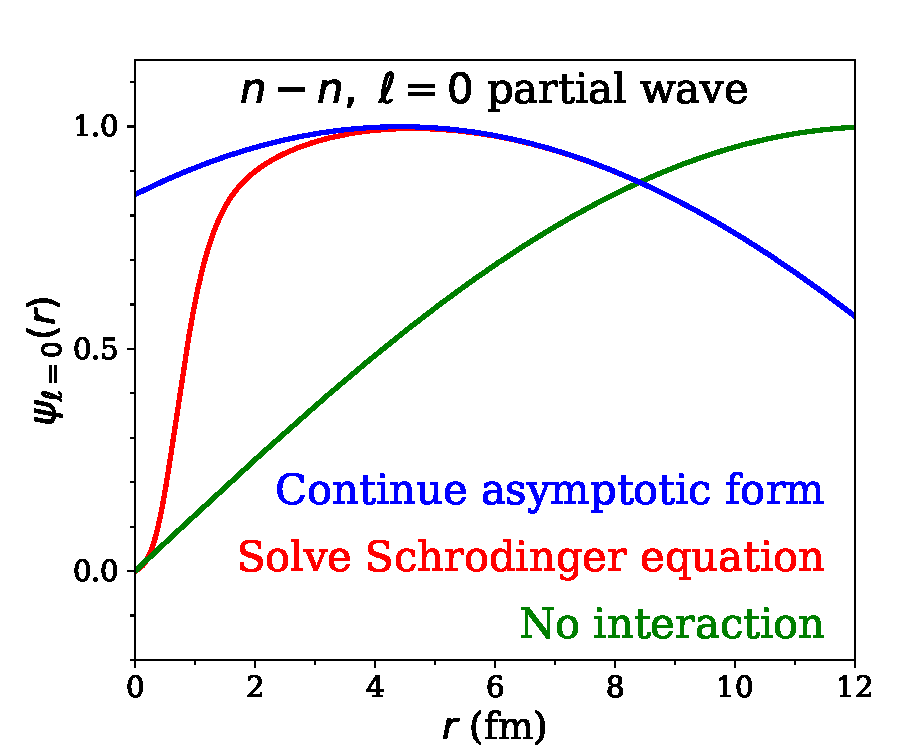
\includegraphics[width=0.6\textwidth]{nnwf}}
\caption{\label{fig:nnwf}
The $n-n$ partial wave behaves as $\sin(kr)$ in the absence of a potential (green). Adding the potential and solving the Schrodinger equation results in a wave function with additional strength near the origin (red). As an approximation, one can use the asymptotic form, $\sin(kr+\delta)$ (blue). This depends only on the phase shift. This simplifies the equation, but is a poor approximation for $r<2 fm$, which would lead to poor predictions of correlation functions if source sizes are small.}
\end{figure}
Unlike the extension of the form in Eq. (\ref{eq:assform}), the true wave function disappears at $r=0$. As an example, Fig. \ref{fig:nnwf} shows the difference between the full solution of the partial wave, which involves solving the Schrodinger equation numerically, to simply using the asymptotic form, $\sin(kr+\delta)$, which can be accounted for by any expression for the phase shift. Experimental phase shifts or effective range expansions can be used here.

The asymptotic form becomes exact when outside the range of the potential. For the $n-n$ example this was around 2 fm, but for any wave function involving deuterons, that range becomes much larger due to the size of the deuteron. Any use of the asymptotic form then becomes quite unreasonable.

The advantage of applying the asymptotic form is only in its ease of use. For Gaussian shapes, one can perform integrals analytically, avoiding the need to numerically calculate integrals. However, calculating wavefunctions at 100,000, which gives very smooth correlation functions, for each of 80 momenta, i.e. 8 millions wave functions, is finished under 5 seconds on a laptop using CorAL. So, the main advantage is in the avoidance of tuning potentials to reproduce phase shifts, rather than the CPU usage of calculating wave functions.


\section{Sensitivity to Exact Form of Potential}

Any number of potentials can fit a given set of phase shifts. Thus, it raises the question of whether the specific form of the potential might make a difference. Here, I make the case that any potential that reproduces the phase shifts, as long as the range is not unreasonable, should give close to the same answer.

For calculating a wavefunction for use in Eq. (\ref{eq:koonin}), one need only know the phaseshifts when $r$ is larger than the range of the potential. For the $n-n$ case above the range is $\approx 2$ fm. For smaller radii, it is worthwhile noting the \href{https://journals.aps.org/pr/abstract/10.1103/PhysRev.76.38}{sum rule},
\begin{align*}\eqnumber
\int_0^\infty dr~e^{-\epsilon r}\left[ |\phi_{q}(r)|^2-\sin^2(qr)\right]&=\frac{1}{2}\frac{d\delta}{dk}.
\end{align*}
where $\epsilon\rightarrow 0$. This works for ANY potential. Because the exact form of the potential does not affect the integral for $r$ outside the range of the potential, and because the integrated strength of $|\phi_q(r)|^2$ is independent of the exact form (as long as the potential reproduces both $\delta(q)$ and $d\delta/dq$), that there is no way for the integral in Eq. (\ref{eq:koonin}) to change significantly unless the source function changes significantly inside the range of the potential. Thus, any two potentials that reproduce the phase shifts should result in nearly identical correlation functions using Eq. (\ref{eq:koonin}). The only way that a sensitivity might ensue would be if the source function inside the range of the potential varied so much that shuffling the strength of $|\phi_q(r)|^2$ within that range might affect the integral.


\end{document}